\documentclass[14pt]{extarticle}
\usepackage[margin=1in]{geometry}
\usepackage{amsmath}
\usepackage{listings}
\usepackage{xcolor}
\usepackage{graphicx}
\usepackage{tcolorbox}
\usepackage{multicol}
\usepackage{titlesec}
\usepackage{enumitem}
\usepackage{makecell}
\usepackage{tikz}
\usetikzlibrary{positioning, arrows.meta}


\definecolor{codegray}{gray}{0.95}
\lstset{
    basicstyle=\ttfamily\small,
    frame=single,
    breaklines=true,
    columns=fullflexible,
}

\title{\textbf{Selection Sort}}
\author{Varun Kumar}
\date{July 4, 2025}

\begin{document}

\maketitle

\section*{1. Logic}

Selection Sort repeatedly finds the minimum element from the unsorted part of the array and puts it at the beginning.

\begin{tcolorbox}[
  colback=white,
  colframe=black,
  title=Key Idea
]
At the $i^{th}$ iteration, the smallest element from index $i$ to $n-1$ is selected and swapped with the element at index $i$.
\end{tcolorbox}

\section*{2. Number of Comparisons and Swaps}

Let $n$ be the number of elements.

\subsection*{Worst, Best, and Average Case}

\begin{itemize}
    \item Comparisons: $\frac{n(n-1)}{2}$
    \item Swaps: $n - 1$
\end{itemize}

\section*{3. Optimal Behavior}

Selection Sort does not adapt to the input data. It performs the same number of comparisons regardless of the input's order.

\section*{4. Pseudocode}

\begin{lstlisting}[language=Python]
function selectionSort(arr):
    n = length(arr)
    for i = 0 to n-2:
        min_idx = i
        for j = i+1 to n-1:
            if arr[j] < arr[min_idx]:
                min_idx = j
        swap arr[i] and arr[min_idx]
\end{lstlisting}

\begin{tcolorbox}[
  colback=white,
  colframe=black,
  title=Stability Note
]
Selection Sort is not stable because it may change the relative order of equal elements due to swapping.
\end{tcolorbox}

\section*{5. Example Walkthrough}

Given: \texttt{[5, 1, 4, 2, 8]}

\subsection*{Pass 1}
Find min from index 0 to 4 → 1  
Swap 5 and 1 → \texttt{[1, 5, 4, 2, 8]}

\subsection*{Pass 2}
Find min from index 1 to 4 → 2  
Swap 5 and 2 → \texttt{[1, 2, 4, 5, 8]}

\subsection*{Pass 3}
Find min from index 2 to 4 → 4  
Already in position → No swap

\subsection*{Pass 4}
Find min from index 3 to 4 → 5  
Already in position → No swap

\section*{6. Mixed Case Behavior in Selection Sort}

Input Array:
\begin{lstlisting}[language=Python]
[(1, 'A'), (3, 'B'), (5, 'C'), (2, 'D'), (4, 'E')]
\end{lstlisting}

This example includes both:
\begin{itemize}
    \item \textbf{Best-case behavior:} some elements (e.g., (1, 'A')) are already in the correct position.
    \item \textbf{Worst-case behavior:} some elements (e.g., (5, 'C')) need to move far.
\end{itemize}

\subsection*{Pass 1 (i = 0)}
Find min from index 0 to 4 → (1, 'A') (already in correct position)

\textbf{No shift performed.}

\begin{lstlisting}[language=Python]
[(1, 'A'), (3, 'B'), (5, 'C'), (2, 'D'), (4, 'E')]
\end{lstlisting}

\subsection*{Pass 2 (i = 1)}
Find min from index 1 to 4 → (2, 'D')

Insert it at index 1 by shifting right:

\begin{lstlisting}[language=Python]
[(1, 'A'), (2, 'D'), (3, 'B'), (5, 'C'), (4, 'E')]
\end{lstlisting}

\subsection*{Visual for Pass 2 (Insert (2, 'D'))}

\begin{center}
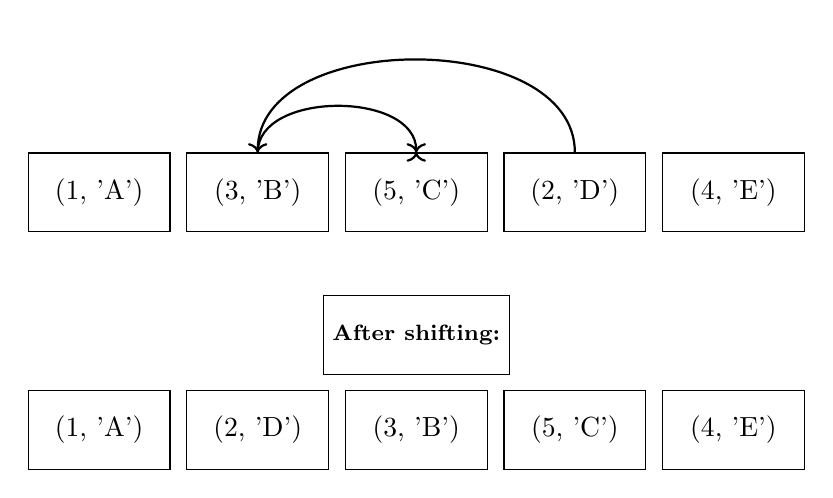
\begin{tikzpicture}[every node/.style={rectangle, draw, minimum height=1cm, minimum width=1.8cm}, node distance=0.2cm]
\node (a0) {(1, 'A')};
\node (a1) [right=of a0] {(3, 'B')};
\node (a2) [right=of a1] {(5, 'C')};
\node (a3) [right=of a2] {(2, 'D')};
\node (a4) [right=of a3] {(4, 'E')};

% Arrows for shifting
\draw[->, thick] (a3.north) to[out=90,in=90] (a1.north);
\draw[->, thick] (a2.north) to[out=90,in=90] (a2.north);
\draw[->, thick] (a1.north) to[out=90,in=90] (a2.north);

% Label
\node (label) [below=0.8cm of a2, font=\footnotesize\bfseries] {\textbf{After shifting:}};

% After state
\node (b0) [below=2cm of a0] {(1, 'A')};
\node (b1) [right=of b0] {(2, 'D')};
\node (b2) [right=of b1] {(3, 'B')};
\node (b3) [right=of b2] {(5, 'C')};
\node (b4) [right=of b3] {(4, 'E')};

\end{tikzpicture}
\end{center}

\begin{tcolorbox}[colback=white, colframe=black, title=What Happened]
(2, 'D') was the minimum from index 1 to 4.  
Instead of swapping directly with (3, 'B'), we shifted (3, 'B') and (5, 'C') one step to the right, and inserted (2, 'D') at index 1.  
This preserved the relative order → \textbf{stable sort}.
\end{tcolorbox}


\subsection*{Pass 3 (i = 2)}
Find min from index 2 to 4 → (3, 'B') (already in correct position)

\textbf{No shift performed.}

\begin{lstlisting}[language=Python]
[(1, 'A'), (2, 'D'), (3, 'B'), (5, 'C'), (4, 'E')]
\end{lstlisting}

\subsection*{Pass 4 (i = 3)}
Find min from index 3 to 4 → (4, 'E')

Shift and insert at index 3:

\begin{lstlisting}[language=Python]
[(1, 'A'), (2, 'D'), (3, 'B'), (4, 'E'), (5, 'C')]
\end{lstlisting}

\subsection*{Pass 5 (i = 4)}
Only one element remains → Done.

\subsection*{Final Sorted Output}

\begin{lstlisting}[language=Python]
[(1, 'A'), (2, 'D'), (3, 'B'), (4, 'E'), (5, 'C')]
\end{lstlisting}

\begin{tcolorbox}[colback=white, colframe=black, title=Summary of Mixed Behavior]
\begin{itemize}
    \item (1, 'A') and (3, 'B') were already in place → \textbf{Best-case behavior}.
    \item (5, 'C') moved from index 2 to 4 → \textbf{Worst-case behavior}.
\end{itemize}
This demonstrates both behaviors in the same execution.
\end{tcolorbox}


\section*{7. Python Code with Explanation}

\begin{lstlisting}[language=Python]
def selection_sort(arr):
    n = len(arr)  # Get the length of the array

    # Traverse the array from index 0 to n-2
    for i in range(n - 1):
        min_idx = i  # Assume the minimum is at the current index

        # Find the index of the minimum element in the unsorted part
        for j in range(i + 1, n):
            if arr[j] < arr[min_idx]:
	        # Update min_idx if a smaller element is found
                min_idx = j  

        # Swap the found minimum element with the element
        # at the current index i
        arr[i], arr[min_idx] = arr[min_idx], arr[i]

    return arr  # Return the sorted array
\end{lstlisting}

\newpage
\section*{8. Why is Selection Sort Unstable?}

Selection Sort is \textbf{unstable} because it swaps elements even when their keys are equal, which can change the original relative order of those elements.

\subsection*{Illustration with an Example}

Consider the array of tuples where each tuple contains a key and a label:

\begin{lstlisting}[language=Python]
arr = [(4, 'A'), (4, 'B'), (3, 'C')]
\end{lstlisting}

\textbf{Step 1:} Find the minimum element → $(3, 'C')$

\textbf{Step 2:} Swap it with the first element → $(4, 'A')$

Resulting array:

\begin{lstlisting}[language=Python]
[(3, 'C'), (4, 'B'), (4, 'A')]
\end{lstlisting}

Now, the element $(4, 'A')$ comes \textbf{after} $(4, 'B')$, even though originally it appeared \textbf{before}. This violates the principle of \textit{stability}, where equal keys must retain their input order.

\subsection*{Why This Happens in Logic}

In the core logic of selection sort:
\begin{lstlisting}[language=Python]
arr[i], arr[min_idx] = arr[min_idx], arr[i]
\end{lstlisting}

This line swaps unconditionally, without checking if the elements are equal, thus potentially breaking the original order.

\begin{tcolorbox}[
  colback=white,
  colframe=black,
  title=Summary
]
Selection Sort is not stable because it uses direct swapping, which may reorder equal elements and break their original sequence.
\end{tcolorbox}

\newpage
\section*{9. Making Selection Sort Stable}

Selection Sort can be made \textbf{stable} by avoiding direct swapping. Instead of swapping the minimum element with the current index, we \textbf{shift} all elements to the right and \textbf{insert} the minimum element at its correct position.

\subsection*{Stable Selection Sort Logic}

\begin{tcolorbox}[
  colback=white,
  colframe=black,
  title=Key Idea
]
Instead of swapping the minimum element directly with the current index, store the minimum, shift the intermediate elements to the right, and insert the minimum value at the correct index.
\end{tcolorbox}

\subsection*{Stable Selection Sort Code (Python)}

\begin{lstlisting}[language=Python]
def stable_selection_sort(arr):
    n = len(arr)
    for i in range(n):
        min_idx = i
        for j in range(i + 1, n):
            if arr[j] < arr[min_idx]:
                min_idx = j

        # Store the minimum element
        key = arr[min_idx]

        # Shift all elements between i and min_idx to the right
        while min_idx > i:
            arr[min_idx] = arr[min_idx - 1]
            min_idx -= 1

        # Insert the minimum element at its correct position
        arr[i] = key
\end{lstlisting}

\begin{tcolorbox}[
  colback=white,
  colframe=black,
  title=Result
]
This version of Selection Sort is \textbf{stable} and maintains the relative order of equal elements.
\end{tcolorbox}

\section*{10. Example Walkthrough of Stable Selection Sort}

\textbf{Initial Array:}

\begin{lstlisting}[language=Python]
[(4, 'A'), (5, 'B'), (3, 'C'), (4, 'D'), (1, 'E'), (2, 'F'), (6, 'G')]
\end{lstlisting}

\subsection*{Pass 1 (i = 0)}
Find minimum from index 0 to 6 → (1, 'E')

Insert it at index 0 by shifting others right:

\begin{lstlisting}[language=Python]
[(1, 'E'), (4, 'A'), (5, 'B'), (3, 'C'), (4, 'D'), (2, 'F'), (6, 'G')]
\end{lstlisting}

\subsection*{Pass 2 (i = 1)}
Find minimum from index 1 to 6 → (2, 'F')

Shift and insert:

\begin{lstlisting}[language=Python]
[(1, 'E'), (2, 'F'), (4, 'A'), (5, 'B'), (3, 'C'), (4, 'D'), (6, 'G')]
\end{lstlisting}

\subsection*{Pass 3 (i = 2)}
Find minimum from index 2 to 6 → (3, 'C')

Shift and insert:

\begin{lstlisting}[language=Python]
[(1, 'E'), (2, 'F'), (3, 'C'), (4, 'A'), (5, 'B'), (4, 'D'), (6, 'G')]
\end{lstlisting}

\subsection*{Pass 4 (i = 3)}
Find minimum from index 3 to 6 → (4, 'A') (already in place)

No shift needed.

\begin{lstlisting}[language=Python]
[(1, 'E'), (2, 'F'), (3, 'C'), (4, 'A'), (5, 'B'), (4, 'D'), (6, 'G')]
\end{lstlisting}

\subsection*{Pass 5 (i = 4)}
Find minimum from index 4 to 6 → (4, 'D')

Shift and insert:

\begin{lstlisting}[language=Python]
[(1, 'E'), (2, 'F'), (3, 'C'), (4, 'A'), (4, 'D'), (5, 'B'), (6, 'G')]
\end{lstlisting}

\subsection*{Pass 6 (i = 5)}
Find minimum from index 5 to 6 → (5, 'B') (already in place)

\begin{lstlisting}[language=Python]
[(1, 'E'), (2, 'F'), (3, 'C'), (4, 'A'), (4, 'D'), (5, 'B'), (6, 'G')]
\end{lstlisting}

\subsection*{Pass 7 (i = 6)}
Only one element left → Done.

\subsection*{Final Output}
\begin{lstlisting}[language=Python]
[(1, 'E'), (2, 'F'), (3, 'C'), (4, 'A'), (4, 'D'), (5, 'B'), (6, 'G')]
\end{lstlisting}

\begin{tcolorbox}[colback=white, colframe=black, title=Stability Observed]
(4, 'A') came before (4, 'D') and remains in that order after sorting. Hence, the algorithm is stable.
\end{tcolorbox}

\newpage
\section*{11. Best and Worst Case of Selection Sort}

Selection Sort is \textbf{not adaptive}, which means it performs the same number of comparisons regardless of the input order.

\subsection*{Best Case}
\begin{itemize}
    \item \textbf{Input:} Already sorted array \texttt{[1, 2, 3, 4, 5]}
    \item \textbf{Comparisons:} Always $\frac{n(n - 1)}{2}$
    \item \textbf{Swaps:} Exactly $n - 1$, even if elements are already in place \\
          (can be reduced with optimization to skip unnecessary swaps)
\end{itemize}

\textbf{Time Complexity:} $O(n^2)$ \\
\textbf{Swaps:} $O(n)$

\vspace{1em}

\subsection*{Worst Case}
\begin{itemize}
    \item \textbf{Input:} Reverse sorted array \texttt{[5, 4, 3, 2, 1]}
    \item \textbf{Comparisons:} Still $\frac{n(n - 1)}{2}$
    \item \textbf{Swaps:} $n - 1$
\end{itemize}

\textbf{Time Complexity:} $O(n^2)$ \\
\textbf{Swaps:} $O(n)$

\vspace{1em}

\subsection*{Summary Table}

\begin{center}
\renewcommand{\arraystretch}{1.3}
\begin{tabular}{|c|c|c|c|c|c|}
\hline
\textbf{Case} & \textbf{Comparisons} & \textbf{Swaps} & \textbf{Time} & \textbf{Adaptive} & \textbf{Stable} \\
\hline
Best Case & $\frac{n(n - 1)}{2}$ & $n - 1$ & $O(n^2)$ & \textcolor{red}{No} & \textcolor{red}{No} \\
Worst Case & $\frac{n(n - 1)}{2}$ & $n - 1$ & $O(n^2)$ & \textcolor{red}{No} & \textcolor{red}{No} \\
\hline
\end{tabular}
\end{center}

\vspace{1em}

\begin{tcolorbox}[colback=white, colframe=black, title=Note]
\begin{itemize}
    \item The number of comparisons is always the same: $\frac{n(n-1)}{2}$.
    \item Selection Sort is useful when:
    \begin{itemize}
        \item Swaps are expensive (since it does at most $n - 1$ swaps).
        \item Simplicity or small input size is acceptable.
    \end{itemize}
\end{itemize}
\end{tcolorbox}


\section*{12. Time \& Space Complexity and Its Properties}

\begin{center}
\begin{tabular}{|l|l||l|l|}
\hline
\textbf{Case}     & \textbf{Complexity}   & \textbf{Property}     & \textbf{Value} \\
\hline
Best Case         & $O(n^2)$              & Stable                & No             \\
Average Case      & $O(n^2)$              & In-place              & Yes            \\
Worst Case        & $O(n^2)$              & Adaptive              & No             \\
\hline
\noalign{\vskip 2pt}
Space Complexity  & $O(1)$ (in-place)     & Recursive             & No             \\
\hline
\end{tabular}
\end{center}

\end{document}
